% !TeX program = latexmk
% !TeX spellcheck = pl_PL
% !TeX root = example.tex

\chapter{Wprowadzenie}

Najpopularniejszą definicją projektu jest definicja Project Management Institute (PMI – międzynarodowe stowarzyszenie zrzeszające kierowników projektów.
Project Management Institute powstał w 1969 w Pensylwanii w USA jako stowarzyszenie non profit zrzeszające profesjonalistów
w dziedzinie zarządzania projektami- istnieje również oddział we Wrocławiu.): 
\begin{quote}
Projekt, to tymczasowa działalność podejmowana w celu wytworzenia unikatowego wyrobu,
dostarczenia unikatowej usługi lub otrzymania unikatowego rezultatu
\end{quote}
~\cite{PMI_2000}
Już w starożytnym Egipcie istniały metody zarządzania skomplikowanym przedsięwzięciem,
np budowa piramid. Było to olbrzymie wyzwanie, które wymagało wiedzy zarówno planistycznej,
jak i logistycznej. W ubiegłym stuleciu, w latach 50 stosowano podejścia zwane obecnie współczesnymi
technikami zarządzania projektami. Weźmy np projekt systemu rakiet balistycznych Polaris.
Okazał się on swoistym koszmarem technicznym i administracyjnym. Nad projektem pracowała olbrzymia ilość zespołów badawczych,
projektowych i produkcyjnych. Dla udokumentowania wszystkich działań zużyto tony papieru, a samo zarządzanie projektami zaczęto
uznawać za dziedzinę bardzo skomplikowaną, niedostępną, opartą na wiedzy specjalistów.\cite{Stanley_2013}

\section{Najpopularniejsze metody zarządzania projektami}
Przy dokonywaniu wyboru metodyki zarządzania projektem należy przeprowadzić adekwatną analizę w celu doboru odpowiedniego podejścia,
gdyż każda z metodyk posiada wady i zalety. Wyróżniamy dwa podejścia (klasyczne i zwinne), które różnią się dość mocno między sobą w kilku płaszczyznach (przekrojach),takich jak:
odpowiedzialność za produkt, rola menedżera w zespole, istota prac wstępnych, zdefiniowanie produktu czy odpowiedź zwrotna użytkowników.
Co uwzględniono w tabeli \~ref{tabela:roznice}.

% Tabela. Nazwa tabeli u góry.
\begin{table}
\centering\caption{ Różnice między podejściem klasycznym a zwinnym\label{tabela:roznice}}
\begin{tabular}{ p{0.25\textwidth} p{0.3\textwidth}  p{0.3\textwidth} }% wyrównanie kolumn tabeli -> l c r - do lewej, środka, do prawej
\toprule
\textbf{Płaszczyzna} &\textbf{ Podejście klasyczne} & \textbf{Podejście zwinne} \\
\midrule
\textbf{Odpowiedzialność
za produkt}
 & Podzielona między marketera,
 menadżera produktu i menadżera projektu & Istnieje tylko jeden właściciel produktu \\
\midrule
\textbf{Rola menedżera
w zespole} & oddzielony od zespołów deweloperskich & Jest członkiem zespołu i ściśle z nim współpracuje.\\
\midrule
\textbf{Istota prac wstępnych} & Przeprowadzane są szczegółowe badania rynku, planowanie produktu i analizy biznesowe
& Ograniczają się do stworzenia wizji, która ogólnie opisuje wygląd i działanie produktu. \\
\midrule
\textbf{Zdefiniowanie
produktu} & Wymagania są określane i zatwierdzane w początkowej fazie
& Produkt odkrywany jest stopniowo, a wymagania krystalizują się w trakcie
\\
\midrule
\textbf{Odpowiedź zwrotna} & Dostępna po wypuszczeniu produktu na rynek
& Wczesna i częsta odpowiedź zwrotna po małych wdrożeniach
\\
\bottomrule
\end{tabular}
\end{table}
\newpage

\section{Podejście klasyczne}

Podejście klasyczne, reprezentowane przez PMBoK (Kompendium wiedzy o zarządzaniu projektami) lub metodykę PRINCE
(kompleksowa metodą zarządzania projektami, zalicza się ją do podejścia klasycznego) oraz jej następcę PRINCE2,
ma na celu wytworzenie kompletnego produktu przy uprzednim, dokładnym określeniu jego cech.
Takie podejście charakteryzuje się ogromnym formalizmem, weźmy na przykład dokonywanie zmian,
które wiąże się z wypełnianiem dokumentów (RfC – ang. Request for Change) -prośby o zmianę.
Każda odpowiedź, to z kolei oczekiwanie, aż zostanie przeanalizowana i zatwierdzona bądź odrzucona.
Dodatkowo osoby odpowiedzialne zwykle nie pracują wraz z zespołem, w związku z czym często występują bariery komunikacyjne.\cite{www_tradycyjne_projekty}

\section{Podejście zwinne}

Podejście zwinne ukierunkowane jest na zespół, który w pełni odpowiada za wykonanie swojej części
zadania i stopniowo dostosowuje je do potrzeb przyszłych użytkowników. Przykładowe metodyki zwinne,
to m.in.: Scrum, Lean, Cobit, SixSigma, Kanban, XP (ang eXtream Programming), TDD (ang. Test-Driven Development)
i FDD (ang. Feature-Driven Development).
W praktycznej działalności często zespoły nie wykorzystują jednej metodyki, a opierają się na kilku.
Przykładem może być tutaj niedawno powstały Scrum-ban, który jest połączeniem dobrych praktyk zaczerpniętych ze Scruma i Kanbana.
~\cite{Wolf_2012} Ciekawym rozwiązaniem jest także TDD, czyli programowanie sterowane testami. Proponuje ono utworzenie przypadków testowych,
zanim powstanie fragment kod.\cite{TDD_2015} 
Każde z prezentowanych rozwiązań posiada swoje zalety,
jednak najważniejsze jest dobranie odpowiedniej metodyki do realiów pracy i prawidłowa adaptacja względem realiów biznesowych,
gdyż ścisłe stosowanie wszystkich praktyk może być nadmiernie pracochłonne w zastosowaniu do małych projektów.

\section{Manifest Agile}

Manifest Agile powstał w 2001 roku, ale nie jest to sam początek tego ruchu zwinnego oprogramowania. Już wcześniej istniały pewne metodyki, jak również istniały podstawy teoretyczne dla wprowadzenia takich rozwiązań. Jeśli chodzi o podstawy teoretyczne, to trzeba zwrócić uwagę przede wszystkim na 3 kwestie:
	\begin{itemize}
		\item kwestię podejścia systemowego i szkoły systemowej (czyli lata 70-te XX w.),
		która dostarczyła dość znaczącej wiedzy pozwalającej na współczesne zarządzanie projektami;
		\item drugi aspekt, to zarządzanie jakością, koncepcje, metody zarządzania jakością, które są wykorzystywane bardzo mocno w metodykach zwinnych;
		\item trzeci aspekt, to zarządzanie wiedzą, czyli chociażby Takeuchi i Nonaka,
		którzy jako pierwsi wspomnieli o idei młyna (w artykule The new product development game,
		opublikowanym w „Harvard Business Review” w 1986 r.), skąd wzięła się później metoda „scrum”.
	\end{itemize}
W latach 90-tych zaobserwowano znaczące skomplikowanie oprogramowania, tworzenia oprogramowania.
Projekty dotychczas zarządzane klasycznie okazały się zbyt mało elastyczne, nie pozwalały na wystarczająco szybkie tworzenie oprogramowania.
Zdecydowano więc, że trzeba jakoś zmodyfikować sposób, w jaki tworzymy oprogramowanie, aby odpowiadać na potrzeby klientów,
na potrzeby rynku wystarczająco szybko. Pierwsze próby podjęto już na początku lat 90-tych XX w. Zostały one uwieńczone publikacją w 1995 r.
metodyki scrum, opisu, w jaki sposób można stosować tą metodykę. Rok później pojawiła się Metodyka Extreme Programming,
a więc już w połowie lat 90-tych mieliśmy metodyki zwinne, które stosowane były najpierw w ograniczonym zakresie, potem coraz szerzej.
Również poszczególne organizacje, przedsiębiorstwa zaczęły tworzyć swoje odmiany tych metod.
Tak więc dziś mamy całe bogactwo metodyk związanych z zarządzaniem zwinnym w projektach.
Agile nie było zatem pierwsze, było po prostu pewnym podsumowaniem pierwszego etapu rozwoju tych metodyk zwinnych.
W 2001r powstał Manifest, który określił, co jest ważne w zwinnym zarządzaniu projektem. 
~rys\ref{rys:agile}

\begin{figure}
	\centering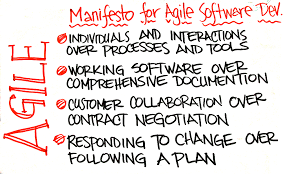
\includegraphics[width=.6\textwidth]{img/agile}
	\caption{Manifesto for Agile Software Dev.[www.medium.com]}.\label{rys:agile}% Źródło rysunku i etykieta przez którą odwołujemy się do rysunku.
\end{figure}

\newpage

Ten Manifest pokazywał pewien system wartości, co jest ważniejsze, a co mniej ważne w zarządzaniu projektem. Mamy więc takie cztery porównania:

\begin{itemize}
	\item Autorzy Manifestu twierdzili, że ludzie i interakcje między nimi są ważniejsi, niż procesy i narzędzia- to nie znaczy, że procesy i narzędzia nie są istotne, ale są mniej istotne, mniej ważne. Trzeba położyć większy nacisk na ludzi, na interakcje- to powoduje bardziej nieformalną komunikację, jej przyspieszenie, również przyspieszenie realizowania zadań i umożliwia bardziej elastyczne realizowanie tych zadań, kiedy zmieniają się warunki;
	\item Druga zasadą jest orientacja bardziej na działające oprogramowanie, niż na dokumentację. Jeśli zerkniemy do starych wersji oprogramowania z lat 80-tych, 90-tych, do każdego programu dodawana była gruba instrukcja. Dzisiaj już o tym zapomnieliśmy. Dzisiaj wiele aplikacji nie ma w ogóle nawet instrukcji- mówimy, że działają intuicyjnie (przynajmniej powinny). Dzięki temu, że orientujemy się na realizację tych najważniejszych efektów w projekcie, możemy lepiej wykorzystać zasoby, możemy szybciej osiągnąć te efekty, a rzeczy mniej ważne, mniej istotne, takie właśnie, jak szczegółowa dokumentacja (jakaś dokumentacja przecież musi być), możemy odłożyć, możemy przeznaczyć dla nich mniejsze zasoby.
	\item Również jeśli chodzi o współpracę z klientem, w metodykach zwinnych proponuje się zmianę podejścia. Zamiast negocjować szczegółowo umowy, budujemy współpracę z tym klientem dlatego, że nie jesteśmy w stanie z góry przewidzieć, jaki będzie, tak do końca, zakres naszego projektu, co w tym projekcie zrealizujemy, co będzie potrzebne za rok, kiedy nasz produkt będzie prawie gotowy. Czy te wymagania się nie zmienią wielokrotnie, biorąc pod uwagę szybkość zmiany technologii, potrzeb, oczekiwań klientów, szybkość zmian na rynku. Zatem klient powinien być blisko, powinien dostarczać bieżące informacje o swoich potrzebach, a w kontrakcie zawieramy tylko te informacje, które są najważniejsze.
	\item I w końcu reagowanie na zmiany zamiast szczegółowego planowania.
	Oczywiście planowanie występuje w metodykach zwinnych, ale jest ono ograniczone tylko do tego, żeby dało się zarządzać takim projektem. Natomiast przede wszystkim orientujemy się na reagowanie na zmiany: zmiany potrzeb klienta, zmiany na rynku. Na dostosowanie naszego projektu, w kolejnych iteracjach, do tego, czego klient oczekuje.
\end{itemize}

Czasem niektórzy mówią, może żartobliwie, ale nieraz całkiem serio, że jeżeli czegoś nie zaplanowali, to stosowali właśnie Agile. Nic bardziej błędnego: w Agile każda iteracja jest planowana, w każdym dniu planujemy swoją pracę, stosujemy inne metody, rzadko stosujemy harmonogram Gantta, ale także planujemy te działania. Zatem taki polski Agile („polnische Agile”, jak niektórzy mówią), to przykład niewłaściwego zarządzania przedsięwzięciami i raczej nie należy się tym chwalić.
Warto jednak zauważyć, że nie do każdego projektu możemy zastosować metodyki zwinne. One się lepiej sprawdzają wtedy, kiedy mamy:
\begin{itemize}
	\item bardzo krótkie, napięte terminy;
	\item projekty mają charakter unikatowy;
	\item są skomplikowane.
\end{itemize}

Mamy do zrealizowania coś nowego, nieoczekiwanego i mało czasu. Wtedy ta metodyka zwinna rzeczywiście jest bardziej uzasadniona niż metodyki klasyczne. Stosowanie metodyk zwinnych, szczególnie żądanie tej interakcji między pracownikami ogranicza nam wielkość zespołu, a więc ogranicza nam wielkość projektu. Generalnie metodyki zwinne stosujemy:
\begin{itemize}
	\item w małych i średnich projektach, rzadziej w projektach dużych;
	\item konieczne jest, aby w metodyce zwinnej dostępny był dla nas klient, klient musi się na bieżąco kontaktować z nami i mówić czego potrzebuje, jakie są jego oczekiwania, czy jest zadowolony z tego, co uzyskuje w poszczególnych iteracjach;

	\item tematyka projektu musi być taka, aby klient z każdej iteracji miał jakąś wartość, bowiem staramy się często wypuszczać oprogramowanie, często wprowadzać nowe jego wersje, ale to powoduje, że ta nowa wersja musi dostarczyć jakąś wartość dla klienta.
\end{itemize}
W przypadku oprogramowania jest to oczywiste. W przypadku, kiedy budujemy jakiś budynek, być może Agile wtedy nie jest aż tak przydatny. Trzeba się zastanowić, czy możemy zastosować całą metodykę Agile, czy jak współcześnie w wielu projektach, zastosować ją tylko w odniesieniu do wybranych modułów projektu, tam, gdzie rzeczywiście ma ona zastosowanie.

Więcej informacji można znaleźć w:\cite{Cohen_2006}